\documentclass[11pt]{article}

\usepackage[letterpaper,margin=1in]{geometry}
\usepackage[T1]{fontenc}
\usepackage[charter]{mathdesign}
\usepackage[scaled=0.92]{helvet}
\usepackage{microtype}
\usepackage{amsmath}
\usepackage{bm}
\usepackage{enumitem}
\usepackage{xcolor}
\usepackage{titlesec}
\usepackage{booktabs,tabularx,array}
\usepackage{tikz}
\usepackage[hidelinks]{hyperref}

\definecolor{headblue}{RGB}{24,54,96}
\definecolor{softblue}{RGB}{232,239,248}
\setlength{\parindent}{0pt}
\setlength{\parskip}{6pt}
\setlist{leftmargin=1.4em,topsep=3pt,itemsep=3pt}
\titleformat{\section}{\sffamily\Large\bfseries\color{headblue}}{\thesection}{0.6em}{}
\titlespacing*{\section}{0pt}{18pt}{6pt}
\titleformat{\subsection}{\sffamily\large\bfseries\color{headblue}}{\thesubsection}{0.5em}{}
\titlespacing*{\subsection}{0pt}{12pt}{4pt}
\allowdisplaybreaks

\newcommand{\EIG}{\mathrm{EIG}}
\newcommand{\KL}{\mathrm{KL}}
\newcommand{\Var}{\mathrm{Var}}
\newcommand{\Cov}{\mathrm{Cov}}
\newcommand{\one}{\mathbf{1}}
\newcommand{\lse}{\operatorname{lse}}
\newcommand{\tr}{\operatorname{tr}}
\newcommand{\diag}{\operatorname{diag}}
\newcommand{\softmax}{\operatorname{softmax}}
\newcommand{\Want}{\par\medskip\noindent{\sffamily\bfseries\color{headblue}What we want to show.}\ }
\newcommand{\Steps}{\par\smallskip\noindent{\sffamily\bfseries\color{headblue}Steps.}\par}
\newcommand{\CheckNum}{\par\smallskip\noindent{\sffamily\bfseries\color{headblue}Check with numbers.}\ }
\newcommand{\Code}{\par\smallskip\noindent{\sffamily\bfseries\color{headblue}In the code.}\ }
\newcommand{\Idea}{\par\smallskip\noindent{\sffamily\bfseries\color{headblue}The idea in words.}\ }
\newenvironment{steps}{\begin{enumerate}[label=\textbf{\arabic*.},leftmargin=2em,itemsep=6pt]}{\end{enumerate}}

\begin{document}
\sloppy

\begin{center}
{\sffamily\bfseries\LARGE Intelligent Eyes: The Derivations, One Step at a Time}\\[6pt]
{\sffamily\large A slow companion to the proposal, the derivations note and the code}\\[10pt]
Dawit Chun
\end{center}
\noindent\rule{\textwidth}{0.4pt}

\textbf{How to read this.} Every result has the same four parts.
\begin{itemize}
  \item \emph{What we want to show}: the result in one line.
  \item \emph{Steps}: one small move at a time. Each step says in words why it is allowed.
  \item \emph{Check with numbers}: a tiny example. Every number in these boxes was computed with the project's own code.
  \item \emph{In the code}: the file and function that does it.
\end{itemize}
Sections 1--8 follow the original derivations note. Section 9 derives the four changes made after the first real results. Section 10 says what was dropped and why.

\tableofcontents

% =====================================================================
\section{Notation and setup}

\subsection{What the eyes see}

A \emph{clip} is a short burst of $T$ frames from one camera trap ($T$ is between 1 and 10). Every frame is resized to $448\times448$ pixels.
\begin{itemize}
  \item The \emph{glance} is the whole frame shrunk to $224\times224$ pixels. The frozen encoder sees every frame this way once.
  \item A \emph{crop} is a $224\times224$ square cut out of the $448\times448$ frame, without shrinking. It covers half the width and half the height of the frame, so an object inside it is seen with twice as many pixels in each direction: a $2\times$ zoom.
  \item The 9 crops sit on a $3\times3$ grid. Their top-left corners are at $0$, $\tfrac14$ and $\tfrac12$ of the frame's side, so neighbouring crops overlap. Crops 1, 3, 7 and 9 are the four corners; crop 5 is the centre.
  \item A \emph{look} is one crop of one frame that we decide to encode. It costs one encoder pass, the same as a glance.
\end{itemize}

\begin{center}
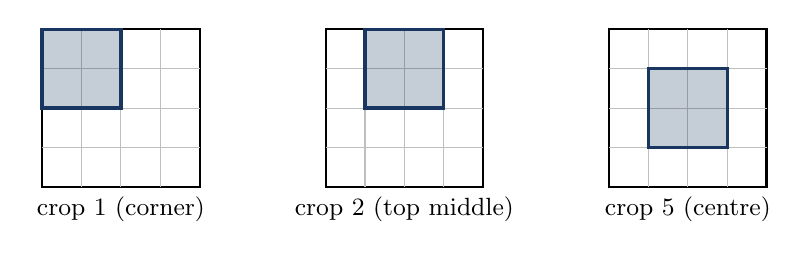
\begin{tikzpicture}[scale=2.0]
  \foreach \x/\lab/\X/\Y in {0/crop 1 (corner)/0/0.5, 1.8/crop 2 (top middle)/0.25/0.5, 3.6/crop 5 (centre)/0.25/0.25} {
    \begin{scope}[xshift=\x cm]
      \draw[thick] (0,0) rectangle (1,1);
      \draw[gray!50] (0.25,0) -- (0.25,1) (0.5,0) -- (0.5,1) (0.75,0) -- (0.75,1);
      \draw[gray!50] (0,0.25) -- (1,0.25) (0,0.5) -- (1,0.5) (0,0.75) -- (1,0.75);
      \fill[headblue,opacity=0.25] (\X,\Y) rectangle ++(0.5,0.5);
      \draw[headblue,very thick] (\X,\Y) rectangle ++(0.5,0.5);
      \node[below] at (0.5,0) {\small \lab};
    \end{scope}
  }
\end{tikzpicture}
\end{center}

We number the 10 \emph{positions} of a frame $k=0,1,\dots,9$: position 0 is the glance and positions $1,\dots,9$ are the crops in reading order. One \emph{observation} is a pair $j=(f,k)$: frame $f$ seen at position $k$.

\subsection{The symbols}

\begin{center}
\small
\begin{tabularx}{\textwidth}{@{}>{\raggedright\arraybackslash}p{2.6cm}X@{}}
\toprule
Symbol & Meaning \\
\midrule
$y$, $K$ & a species, and the number of species \\
$\pi(y)$ & how often species $y$ appears in the training clips (the prior) \\
$T$, $f$, $k$ & number of frames in the clip, a frame index, a position index (0 = glance, 1--9 = crops) \\
$j=(f,k)$ & one observation: frame $f$ at position $k$ \\
$S$ & the set of observations already in the belief (all glances, then the looks that count) \\
$L$ & the looks already taken (a subset of $S$) \\
$q(y\mid x)$ & what a linear classifier on the frozen encoder's feature of image $x$ says about species $y$ \\
$\ell_j(y)$ & the \emph{vote} of observation $j$ for species $y$: $\log q(y\mid x_j)-\log\pi(y)$ \\
$\bm\ell_S$ & the votes of all observations in $S$, stacked (one row per observation) \\
$\mathbf s$ & the score vector of the belief, one number per species \\
$p$ & the belief: $p=\softmax(\mathbf s)$, so $p_y=e^{s_y}/\sum_z e^{s_z}$ \\
$\lse(\mathbf s)$ & ``log-sum-exp'': $\log\sum_y e^{s_y}$ \\
$\one$ & a column of ones \\
$R$ & how much observations repeat each other (a correlation matrix); $R_{SS}$ is its block for $S$ \\
$\bm w$ & the weights $R_{SS}^{-1}\one$: how much each vote counts \\
$n_{\text{eff}}$ & $\one^\top R_{SS}^{-1}\one$: how many independent views the observations are worth \\
$\rho$ & how much the same position repeats from one frame to the next \\
$A$, $A_\lambda$ & the $10\times10$ table of how much two positions in one frame repeat; its shrunk version \\
$\tau$ & the error that all crop votes of a clip share (Section 9c) \\
$\mu_j$, $\sigma^2$ & the predicted vote of a look before taking it, and the size of the prediction error \\
$\bm a_j$, $s_j$, $c_j$ & for a candidate look $j$: what $S$ implies about it, the part of it that is new, and the factor that turns its news into evidence \\
$\Delta_j$, $m_j$, $v_j$ & the change in scores look $j$ would cause, its predicted mean and its variance \\
$F$ & $\diag(p)-pp^\top$, the curvature of $\lse$ \\
$\KL$, $\EIG$, $H(p)$ & KL divergence, expected information gain, entropy of the belief \\
$\varepsilon$ & the stopping threshold \\
$q(\text{empty}\mid c)$ & the crop classifier's probability that crop $c$ shows no animal (Section 9a) \\
\bottomrule
\end{tabularx}
\end{center}

Careful: the letter $s$ is used twice, as in the code. Bold $\mathbf s$ (no subscript) is the score vector. $s_j$ (with a subscript) is the Schur complement of Section 5.

\subsection{Votes}

A classifier says $q(y\mid x)$. The vote subtracts what we believed before seeing anything:
\[ \ell_j(y)=\log q(y\mid x_j)-\log\pi(y). \]
A positive vote means ``after this observation, species $y$ is more likely than it was before''. A negative vote means less likely. A vote of 0 for every species means the observation changed nothing.

\CheckNum $\pi=(0.5,\,0.3,\,0.2)$ and one observation with $q=(0.2,\,0.5,\,0.3)$. The vote is $\log(0.2/0.5)=-0.916$, $\log(0.5/0.3)=0.511$, $\log(0.3/0.2)=0.405$. The first species became less likely, the other two more likely.

\Code \texttt{eyes/belief.py: votes\_\allowbreak{}from\_\allowbreak{}log\_\allowbreak{}probs}; for real clips \texttt{scripts/run\_\allowbreak{}eval.py: votes\_\allowbreak{}for}.

% =====================================================================
\section{Votes add up when observations are independent}

\Want If the observations in $S$ are independent once the species is known, then
\[ \log p(y\mid x_S)=\log\pi(y)+\sum_{j\in S}\ell_j(y)+\text{(a constant that does not depend on }y). \]
\textbf{Assumption (A3).} The classifier is calibrated: $q(y\mid x)$ equals the true probability $p(y\mid x)$.

\Steps
\begin{steps}
  \item Bayes' rule for one observation, using (A3):
  \[ q(y\mid x_j)=\frac{p(x_j\mid y)\,\pi(y)}{p(x_j)}. \]
  \item Divide both sides by $\pi(y)$:
  \[ \frac{q(y\mid x_j)}{\pi(y)}=\frac{p(x_j\mid y)}{p(x_j)}. \]
  \item Take the logarithm of both sides. The left side is the vote:
  \[ \ell_j(y)=\log p(x_j\mid y)-\log p(x_j). \]
  So a vote is a log likelihood ratio: how much better species $y$ explains the image than an average species does.
  \item Bayes' rule for all observations together:
  \[ p(y\mid x_S)=\frac{p(x_S\mid y)\,\pi(y)}{p(x_S)}. \]
  \item Independence given the species means the joint likelihood is a product:
  \[ p(x_S\mid y)=\prod_{j\in S}p(x_j\mid y). \]
  \item Take logs of step 4 and use step 5 (the log of a product is a sum):
  \[ \log p(y\mid x_S)=\log\pi(y)+\sum_{j}\log p(x_j\mid y)-\log p(x_S). \]
  \item Replace each $\log p(x_j\mid y)$ by $\ell_j(y)+\log p(x_j)$ (step 3, rearranged):
  \[ \log p(y\mid x_S)=\log\pi(y)+\sum_{j}\ell_j(y)+\Big[\sum_j\log p(x_j)-\log p(x_S)\Big]. \]
  \item The bracket does not contain $y$, so it is the same for every species. A softmax ignores anything added equally to every species, so
  \[ p(y\mid x_S)=\softmax\Big(\log\pi+\sum_j\ell_j\Big)_y. \]
\end{steps}

\CheckNum $\pi=(0.5,0.3,0.2)$, $q_1=(0.2,0.5,0.3)$, $q_2=(0.25,0.45,0.30)$. The votes are $\ell_1=(-0.916,\,0.511,\,0.405)$ and $\ell_2=(-0.693,\,0.405,\,0.405)$. Then $\softmax(\log\pi+\ell_1+\ell_2)=(0.077,\,0.577,\,0.346)$. Doing Bayes' rule directly with likelihoods proportional to $q_j/\pi$ gives exactly the same $(0.077,\,0.577,\,0.346)$.

\textbf{Why this is not enough.} Two overlapping crops, or the same spot in two nearly identical frames, are not independent. Adding both votes counts the same evidence twice and makes the belief too sure. Section 3 fixes this.

\Code \texttt{eyes/belief.py: scores} with $R=I$ (all weights 1).

% =====================================================================
\section{\texorpdfstring{Correlated votes: the weights $\bm w=R^{-1}\one$ (eq. 1)}{Correlated votes: the weights w (eq. 1)}}

\subsection{The model}

Imagine one perfectly independent view of the clip. Call the evidence it would give $L(y)$. Every real vote is a noisy copy of it:
\[ \ell_j(y)=L(y)+e_j(y). \]
\textbf{Assumption (A2).} For each species $y$, the errors $e_j(y)$ of the observations in $S$ are jointly Gaussian with mean 0 and covariance $\sigma^2R_{SS}$. Different species components are treated as independent of each other.

What $R$ means:
\begin{itemize}
  \item $R_{jj}=1$: each error has the same size $\sigma^2$.
  \item $R_{ij}$ is the correlation of the errors of $i$ and $j$. $R_{ij}=0$: they make unrelated mistakes. $R_{ij}=1$: they make exactly the same mistake, so the second one adds nothing.
\end{itemize}
Below we work with one species component at a time and drop the $(y)$.

\subsection{\texorpdfstring{The best estimate of $L$ (Proposition 3.1)}{The best estimate of L (Proposition 3.1)}}

\Want The best estimate of $L$ and the resulting belief are
\[ \hat L=\frac{\one^\top R^{-1}\bm\ell}{\one^\top R^{-1}\one},\qquad \Var(\hat L)=\frac{\sigma^2}{n_{\text{eff}}},\qquad p(y)\propto\pi(y)\exp\Big(\sum_{j\in S}w_j\,\ell_j(y)\Big),\quad \bm w=R^{-1}\one. \]
(Here $R$ means $R_{SS}$.)

\Steps
\begin{steps}
  \item Write all votes as one vector: $\bm\ell=L\,\one+\bm e$. Each vote is $L$ plus its own error.
  \item The Gaussian density of $\bm e=\bm\ell-L\one$ is largest when this quantity is smallest:
  \[ Q(L)=(\bm\ell-L\one)^\top R^{-1}(\bm\ell-L\one). \]
  (The density is $\exp(-Q/2\sigma^2)$ up to a constant, so the most likely $L$ minimises $Q$.)
  \item Multiply out. $R^{-1}$ is symmetric, so the two cross terms are equal:
  \[ Q(L)=\bm\ell^\top R^{-1}\bm\ell-2L\,\one^\top R^{-1}\bm\ell+L^2\,\one^\top R^{-1}\one. \]
  \item Differentiate with respect to $L$:
  \[ Q'(L)=-2\,\one^\top R^{-1}\bm\ell+2L\,\one^\top R^{-1}\one. \]
  \item Set the derivative to 0 and solve for $L$:
  \[ \hat L=\frac{\one^\top R^{-1}\bm\ell}{\one^\top R^{-1}\one}. \]
  \item Give names to the pieces. Let $\bm w=R^{-1}\one$. Because $R^{-1}$ is symmetric, $\one^\top R^{-1}=\bm w^\top$, so the top is $\bm w^\top\bm\ell=\sum_j w_j\ell_j$. The bottom is $\one^\top\bm w=\sum_jw_j$; call it $n_{\text{eff}}$. So
  \[ \hat L=\frac{\sum_jw_j\ell_j}{n_{\text{eff}}}. \]
  \item The error of the estimate: subtract $L$ and use $\bm\ell=L\one+\bm e$ and $\bm w^\top\one=n_{\text{eff}}$:
  \[ \hat L-L=\frac{\bm w^\top\bm e}{n_{\text{eff}}}. \]
  \item Its variance (a constant vector times $\bm e$ has variance $\bm w^\top\Cov(\bm e)\bm w$):
  \[ \Var(\hat L)=\frac{\bm w^\top(\sigma^2R)\bm w}{n_{\text{eff}}^2}=\frac{\sigma^2\,\one^\top R^{-1}RR^{-1}\one}{n_{\text{eff}}^2}=\frac{\sigma^2\,n_{\text{eff}}}{n_{\text{eff}}^2}=\frac{\sigma^2}{n_{\text{eff}}}. \]
  \item Read it: averaging $n$ independent views each with error $\sigma^2$ gives variance $\sigma^2/n$. So the correlated votes are worth exactly $n_{\text{eff}}$ independent views whose average is $\hat L$.
  \item Now use Section 2 on those $n_{\text{eff}}$ independent views: their votes add up to $n_{\text{eff}}\times\hat L=\sum_jw_j\ell_j$. Therefore
  \[ p(y)\propto\pi(y)\exp\Big(\sum_jw_j\ell_j(y)\Big). \]
  This is eq. (1). Step 10 is the one modelling choice (treat the votes as $n_{\text{eff}}$ independent views); everything before it is exact under (A2).
\end{steps}

\CheckNum Two votes with correlation $r=0.6$. Then
\[ R=\begin{pmatrix}1&0.6\\0.6&1\end{pmatrix},\qquad R^{-1}=\frac{1}{1-0.36}\begin{pmatrix}1&-0.6\\-0.6&1\end{pmatrix},\qquad \bm w=R^{-1}\one=\frac{0.4}{0.64}\one=(0.625,\,0.625). \]
In general $w=\frac{1-r}{1-r^2}=\frac{1}{1+r}$ for each of two votes. So $n_{\text{eff}}=1.25$: two votes that are 60\% the same count as one and a quarter. With votes 2 and 1, $\hat L=1.5$ and the total evidence is $1.875$, not $3$. The code's \texttt{evidence\_\allowbreak{}weights} gives the same $(0.625,\,0.625)$.

\Code \texttt{eyes/correlation.py: evidence\_\allowbreak{}weights} solves $(R+10^{-6}I)\bm w=\one$ (the tiny ridge keeps $R$ invertible); \texttt{eyes/belief.py: scores, posterior}.

\subsection{Feeding the same observation twice changes nothing (Proposition 3.2)}

\Want If observation $i$ is added again as a new observation $j$ (same vote, same row of $R$), the total evidence $E=\one^\top R^{-1}\bm\ell$ and $n_{\text{eff}}$ do not change.

\Steps
\begin{steps}
  \item The copy has $\ell_j=\ell_i$, and its row of $R$ equals row $i$ (including $R_{ij}=1$). Two rows of the new matrix are equal, so it has no inverse. We use the pseudo-inverse $(\cdot)^+$, which is what the ridge in the code tends to.
  \item Write the copying as a matrix. Let $M$ be the identity with an extra last row equal to row $i$ of the identity, $M=\begin{pmatrix}I\\ e_i^\top\end{pmatrix}$. Then the new votes are $M\bm\ell$, the new ones-vector is $M\one$ and the new correlation matrix is $MRM^\top$.
  \item $M$ has independent columns, so $M^+=(M^\top M)^{-1}M^\top$ and therefore $M^+M=I$. In the same way $M^\top(M^\top)^+=I$.
  \item A known rule for pseudo-inverses of a product of full-rank pieces gives $(MRM^\top)^+=(M^\top)^+R^{-1}M^+$.
  \item Put steps 2 and 4 into the evidence:
  \[ E_{\text{new}}=\one^\top M^\top\,(M^\top)^+R^{-1}M^+\,M\bm\ell. \]
  \item Use step 3 twice: $M^\top(M^\top)^+=I$ and $M^+M=I$:
  \[ E_{\text{new}}=\one^\top R^{-1}\bm\ell=E. \]
  \item Replacing $\bm\ell$ by $\one$ in the same lines shows $n_{\text{eff}}$ is unchanged too.
\end{steps}

\CheckNum $R=\begin{pmatrix}1&0.5\\0.5&1\end{pmatrix}$ and votes $(2,1)$ give $E=2.0$ and $n_{\text{eff}}=1.333$. Feeding observation 1 again (votes $(2,1,2)$, a $3\times3$ matrix with two equal rows) gives, with the pseudo-inverse, again $E=2.0$ and $n_{\text{eff}}=1.333$.

\Code \texttt{tests/test\_\allowbreak{}derivations.py: test\_\allowbreak{}repeat\_\allowbreak{}cannot\_\allowbreak{}change\_\allowbreak{}the\_\allowbreak{}answer}.

\subsection{Ten still frames are worth about two (Proposition 3.3)}

\Want For $T$ glances whose errors repeat over time as $\rho^{|f-f'|}$ (an AR(1) correlation),
\[ w_1=w_T=\frac{1}{1+\rho},\qquad w_2=\dots=w_{T-1}=\frac{1-\rho}{1+\rho},\qquad n_{\text{eff}}=\frac{T-(T-2)\rho}{1+\rho}. \]

\Steps
\begin{steps}
  \item The matrix is $(T_\rho)_{ff'}=\rho^{|f-f'|}$: 1 on the diagonal, $\rho$ next to it, $\rho^2$ two away, and so on.
  \item Its inverse has only three non-zero diagonals:
  \[ T_\rho^{-1}=\frac{1}{1-\rho^2}\begin{pmatrix}1&-\rho&&&\\-\rho&1+\rho^2&-\rho&&\\&\ddots&\ddots&\ddots&\\&&-\rho&1+\rho^2&-\rho\\&&&-\rho&1\end{pmatrix}. \]
  \item Check step 2 by multiplying. Row 1 of the inverse times column 1 of $T_\rho$: $(1\cdot1-\rho\cdot\rho)/(1-\rho^2)=1$. Row 1 times column 2: $(1\cdot\rho-\rho\cdot1)/(1-\rho^2)=0$. A middle row times its own column: $(-\rho\cdot\rho+(1+\rho^2)-\rho\cdot\rho)/(1-\rho^2)=(1-\rho^2)/(1-\rho^2)=1$. A middle row $f$ times a column $g<f$: $(-\rho^{f-g}+\rho^{f-g}+\rho^{f-g+2}-\rho^{f-g+2})/(1-\rho^2)=0$. So the product is the identity.
  \item The weights $\bm w=T_\rho^{-1}\one$ are the row sums of the inverse. First and last row:
  \[ \frac{1-\rho}{1-\rho^2}=\frac{1-\rho}{(1-\rho)(1+\rho)}=\frac{1}{1+\rho}. \]
  \item A middle row:
  \[ \frac{-\rho+1+\rho^2-\rho}{1-\rho^2}=\frac{(1-\rho)^2}{(1-\rho)(1+\rho)}=\frac{1-\rho}{1+\rho}. \]
  \item Add all weights (two end rows and $T-2$ middle rows):
  \[ n_{\text{eff}}=\frac{2+(T-2)(1-\rho)}{1+\rho}=\frac{T-(T-2)\rho}{1+\rho}. \]
\end{steps}

\CheckNum For $T=3$, $\rho=0.5$: $(1-\rho^2)\,T_\rho^{-1}=\begin{pmatrix}1&-0.5&0\\-0.5&1.25&-0.5\\0&-0.5&1\end{pmatrix}$, as step 2 says. For $T=10$, $\rho=0.85$: the end weights are $1/1.85=0.541$, the eight middle weights are $0.15/1.85=0.081$, and $n_{\text{eff}}=(10-6.8)/1.85=1.73$. Solving $T_\rho\bm w=\one$ numerically gives the same numbers. With the $\rho=0.74$ fitted on real data (DINOv2), ten frames are worth $n_{\text{eff}}=2.33$ independent frames. Limits: $\rho=0$ gives $T$; $\rho\to1$ gives 1.

\Code \texttt{eyes/correlation.py: frame\_\allowbreak{}correlation, ar1\_\allowbreak{}effective\_\allowbreak{}frames}; tests \texttt{test\_\allowbreak{}ar1\_\allowbreak{}effective\_\allowbreak{}frames}.

% =====================================================================
\section{\texorpdfstring{The shape of $R$ and how it is fitted}{The shape of R and how it is fitted}}

\subsection{\texorpdfstring{$R=T_\rho\otimes A$}{R = T(rho) x A}}

Two observations $(f,k)$ and $(f',k')$ repeat each other by
\[ R_{(f,k),(f',k')}=A_{kk'}\,\rho^{|f-f'|}. \]
In words: how much the two positions overlap inside one frame ($A_{kk'}$), times how much the frames are alike ($\rho^{|f-f'|}$). Listing observations frame by frame (row $f\cdot10+k$), this is the Kronecker product $R=T_\rho\otimes A$: every entry of $T_\rho$ multiplies a whole copy of $A$.

\CheckNum Two frames, two positions, $\rho=0.8$, $A=\begin{pmatrix}1&0.5\\0.5&1\end{pmatrix}$:
\[ T_\rho\otimes A=\begin{pmatrix}1&0.5&0.8&0.4\\0.5&1&0.4&0.8\\0.8&0.4&1&0.5\\0.4&0.8&0.5&1\end{pmatrix}. \]
The top-right block is $0.8\times A$: the same positions one frame apart.

\textbf{Why $R$ is a valid correlation matrix.} The eigenvalues of a Kronecker product are the products of the eigenvalues of the two pieces. $T_\rho$ has positive eigenvalues for $|\rho|<1$ and $A$ is made positive semidefinite (step 5 below), so all products are at least 0.

\subsection{\texorpdfstring{Fitting $A$ and $\rho$ from class-conditional residuals}{Fitting A and rho from class-conditional residuals}}

The fit uses the 10\% of training cameras held out from the classifiers.
\begin{steps}
  \item For each position $k$ and species $y$, average the votes of all held-out frames whose clip is species $y$. This is the typical vote at that position for that species.
  \item Subtract that average from every vote. What is left, the \emph{residual}, is the part of the vote that is noise. (A2) is a statement about this noise.
  \item Centre each residual vector across species (subtract the average of its $K$ components). Adding the same number to every species changes nothing in the belief (Section 7, $F\one=0$), so that part is not counted.
  \item $\hat A_{kk'}$ is the pooled correlation of residuals at positions $k$ and $k'$ of the same frame: multiply them, add over all frames and species components, and divide by the square roots of the two sums of squares.
  \item An estimated table can be slightly invalid because each entry is estimated on its own. Replace negative eigenvalues by a tiny positive number and rescale so the diagonal is 1.
  \item For each lag $d=1,\dots,4$, compute the pooled correlation $\hat c_d$ of residuals at the same position $d$ frames apart in the same clip.
  \item Choose $\rho$ so that $\rho^d$ matches the measured $\hat c_d$, giving more weight to lags with more pairs $n_d$:
  \[ \hat\rho=\arg\min_\rho\sum_d n_d\big(\hat c_d-\rho^d\big)^2. \]
\end{steps}

\CheckNum Steps 1--3 on four votes at one position. Two frames of species 1 vote $(2.0,\,0.1,\,-0.4)$ and $(1.0,\,0.5,\,0.2)$. Their average is $(1.5,\,0.3,\,-0.1)$, so the residuals are $(0.5,\,-0.2,\,-0.3)$ and $(-0.5,\,0.2,\,0.3)$. Each already sums to 0, so step 3 changes nothing here. For the whole procedure: synthetic votes generated with a known $A$ (entries $0.6,\,0.3,\,0.5$) and $\rho=0.7$ give back $\hat A$ with entries $0.600,\,0.296,\,0.515$ and $\hat\rho=0.705$. On real data (DINOv2, final run, seed 0) the measured lag correlations were $0.61,\,0.52,\,0.46,\,0.43$ and the fit gave $\hat\rho=0.74$, whose powers are $0.74,\,0.55,\,0.41,\,0.30$: the real correlation fades more slowly than $\rho^d$, so the AR(1) shape is an approximation.

With gated fusion (Section 9b), steps 1--7 use only the observations that enter the belief.

\Code \texttt{eyes/correlation.py: class\_\allowbreak{}conditional\_\allowbreak{}residuals, fit\_\allowbreak{}A, fit\_\allowbreak{}rho, nearest\_\allowbreak{}correlation}; test \texttt{test\_\allowbreak{}fit\_\allowbreak{}recovers\_\allowbreak{}known\_\allowbreak{}A\_\allowbreak{}and\_\allowbreak{}rho}.

\subsection{\texorpdfstring{Why the geometric $A$ breaks, and the shrinkage $A_\lambda$}{Why the geometric A breaks, and the shrinkage}}

Before any data, a natural choice is to measure how much two positions overlap:
\[ A_{kk'}=\frac{\text{area}(k\cap k')}{\sqrt{\text{area}(k)\,\text{area}(k')}}. \]
This gives glance and crop $0.5$, side neighbours $0.5$, diagonal neighbours $0.25$, and crops two apart $0$.

\Want This $A$ has no inverse, so $\bm w=A^{-1}\one$ makes no sense; shrinking it fixes that.

\Steps
\begin{steps}
  \item Think of each position as a region of the frame. Let $u_k$ be its indicator (1 inside, 0 outside) divided by the square root of its area. Then $A_{kk'}$ is exactly the inner product of $u_k$ and $u_{k'}$: $A$ is a Gram matrix.
  \item The four corner crops 1, 3, 7, 9 do not overlap and together cover the whole frame. So the glance's indicator is the sum of the four corner indicators.
  \item In terms of the $u$'s (the glance has area 1, each corner area $\tfrac14$, so $\sqrt{\text{area}}=\tfrac12$): $u_0=\tfrac12(u_1+u_3+u_7+u_9)$.
  \item One of the vectors is a combination of the others, so their Gram matrix $A$ has a zero eigenvalue. The vector $(-1,\tfrac12,0,\tfrac12,0,0,0,\tfrac12,0,\tfrac12)$ satisfies $A\bm v=0$.
  \item The weights blow up. With a ridge of $10^{-9}$, $\bm w$ gives the glance about $-5\times10^8$ and each corner $+2.5\times10^8$. With the pseudo-inverse the glance and corners get 0, the edge crops 1 and the centre $-1$. Neither is a sensible ``how much each view counts''.
  \item Why the model fails: eq. (1) assumes every vote is a noisy copy of the same $L$. That holds for the same crop in two frames. It does not hold for crops that look at different parts of the frame: they are not copies of each other.
  \item The fix mixes $A$ with the identity:
  \[ A_\lambda=(1-\lambda)A+\lambda I. \]
  Every eigenvalue becomes $(1-\lambda)a_i+\lambda\ge\lambda>0$, so $A_\lambda$ always has an inverse. $\lambda=0$ is the full table; $\lambda=1$ treats the 10 positions of a frame as independent.
  \item $\lambda$ is chosen on held-out cameras by log-likelihood (the belief's probability of the true species, averaged over two cases: glances plus 2 random looks, and all looks).
\end{steps}

\CheckNum Eigenvalues of the geometric $A$: the smallest is $0.0000$. The vector in step 4, normalised, is $(-0.707,\,0.354,\,0,\,0.354,\,0,\,0,\,0,\,0.354,\,0,\,0.354)$, the null vector the code finds. After shrinking: $\lambda=0.3$ gives condition number $9.7$ and glance weight $-1.19$; $\lambda=0.5$ gives glance $-0.37$ and centre $+0.17$; $\lambda=0.7$ makes every weight positive (glance $0.12$, corners $0.77$). On real data $A$ is fitted from residuals (Section 4.2), not from geometry; the final DINOv2 run chose $\lambda=0.6$.

\Code \texttt{eyes/geometry.py: overlap\_\allowbreak{}correlation}; \texttt{eyes/correlation.py: shrink}; \texttt{eyes/fit.py: choose\_\allowbreak{}shrinkage, choose\_\allowbreak{}R}; tests \texttt{test\_\allowbreak{}overlap\_\allowbreak{}table\_\allowbreak{}is\_\allowbreak{}singular\_\allowbreak{}because\_\allowbreak{}corners\_\allowbreak{}tile\_\allowbreak{}the\_\allowbreak{}frame}.

% =====================================================================
\section{Adding one look: the block inverse (Proposition 4.1)}

Let $S$ be the observations already in the belief and $j$ a candidate look. Define four quantities:
\begin{itemize}
  \item $\bm a_j=R_{SS}^{-1}R_{Sj}$: how well $S$ predicts $j$ (a regression of $j$ on $S$);
  \item $s_j=R_{jj}-R_{jS}\bm a_j$: the Schur complement, the part of $j$ that $S$ cannot predict ($R_{jj}=1$ without the shared crop error of Section 9c);
  \item $\delta_j=\ell_j-\bm a_j^\top\bm\ell_S$: the \emph{innovation}, the vote minus what $S$ already implies about it;
  \item $c_j=(1-\one^\top\bm a_j)/s_j$: the factor that turns the innovation into evidence.
\end{itemize}

\Want With $E_S=\one^\top R_{SS}^{-1}\bm\ell_S$ the total evidence,
\[ E_{S\cup j}-E_S=c_j\,\delta_j,\qquad n_{\text{eff}}(S\cup j)-n_{\text{eff}}(S)=\frac{(1-\one^\top\bm a_j)^2}{s_j}. \]

\Steps
\begin{steps}
  \item The correlation matrix of $S$ plus $j$ in blocks:
  \[ \begin{pmatrix}R_{SS}&R_{Sj}\\R_{jS}&R_{jj}\end{pmatrix}. \]
  \item Its inverse (we check it in step 3):
  \[ \begin{pmatrix}R_{SS}^{-1}+\bm a\bm a^\top/s & -\bm a/s\\ -\bm a^\top/s & 1/s\end{pmatrix}\qquad(\bm a=\bm a_j,\ s=s_j). \]
  \item Check by multiplying the matrix of step 1 by this one, block by block, using $R_{SS}\bm a=R_{Sj}$ and $R_{jj}-R_{jS}\bm a=s$:
  \begin{itemize}
    \item top left: $R_{SS}R_{SS}^{-1}+R_{SS}\bm a\bm a^\top/s-R_{Sj}\bm a^\top/s=I+R_{Sj}\bm a^\top/s-R_{Sj}\bm a^\top/s=I$;
    \item top right: $-R_{SS}\bm a/s+R_{Sj}/s=(-R_{Sj}+R_{Sj})/s=0$;
    \item bottom left: $R_{jS}R_{SS}^{-1}+R_{jS}\bm a\bm a^\top/s-R_{jj}\bm a^\top/s=\bm a^\top-\bm a^\top(R_{jj}-R_{jS}\bm a)/s=\bm a^\top-\bm a^\top=0$;
    \item bottom right: $-R_{jS}\bm a/s+R_{jj}/s=s/s=1$.
  \end{itemize}
  \item The new evidence is $(\one^\top,1)$ times the inverse times $(\bm\ell_S;\ell_j)$. Multiply out the four blocks:
  \[ E_{S\cup j}=\one^\top R_{SS}^{-1}\bm\ell_S+\frac{(\one^\top\bm a)(\bm a^\top\bm\ell_S)}{s}-\frac{(\one^\top\bm a)\,\ell_j}{s}-\frac{\bm a^\top\bm\ell_S}{s}+\frac{\ell_j}{s}. \]
  \item The first term is $E_S$.
  \item Group the other four terms. Two of them contain $(\ell_j-\bm a^\top\bm\ell_S)$ with a plus sign, two contain it multiplied by $(\one^\top\bm a)$ with a minus sign:
  \[ \frac{(\ell_j-\bm a^\top\bm\ell_S)-(\one^\top\bm a)(\ell_j-\bm a^\top\bm\ell_S)}{s}=\frac{(1-\one^\top\bm a)\,\delta_j}{s}=c_j\,\delta_j. \]
  \item The same computation with $\bm\ell$ replaced by $\one$ gives the change in $n_{\text{eff}}$: $\delta_j$ becomes $1-\one^\top\bm a$, so the change is $(1-\one^\top\bm a)^2/s$.
\end{steps}

\Idea A new look only adds its \emph{news}: its vote minus what the earlier observations already said about it. A look that is mostly a repeat has a small $s_j$ and a small news part.

\CheckNum $S$ is one glance with vote $2$; the candidate has vote $3$ and correlation $0.5$ with the glance. Then $\bm a=0.5$, $s=1-0.25=0.75$, $c=(1-0.5)/0.75=0.667$, the innovation is $3-0.5\times2=2$, and the shift is $0.667\times2=1.333$. The evidence goes from $2$ to $3.333$. Computing $\one^\top R^{-1}(2,3)$ directly for $R=\begin{pmatrix}1&0.5\\0.5&1\end{pmatrix}$ also gives $3.333$. With one earlier look of correlation $r$, $c_j=1/(1+r)$, matching the two-vote example of Section 3.

\Code \texttt{eyes/belief.py: add\_\allowbreak{}one\_\allowbreak{}look\_\allowbreak{}terms} (one linear solve for all candidates at once); \texttt{eyes/controller.py: candidate\_\allowbreak{}terms} computes \texttt{implied} $=\bm a^\top\bm\ell_S$ and \texttt{shift} $=c(\ell-\text{implied})$; test \texttt{test\_\allowbreak{}block\_\allowbreak{}inverse\_\allowbreak{}update\_\allowbreak{}matches\_\allowbreak{}recomputation}.

% =====================================================================
\section{Predicting a look before taking it (eq. 2)}

\subsection{The ridge predictor}

For a candidate crop $(f,k)$ the input is $x_j=[\bar u_{fk};\,g_f]$: the average of the glance's own patch tokens inside crop $k$ (a cheap blurry preview of the crop) next to frame $f$'s glance feature. In the final method a third piece is added: what a classifier on $\bar u_{fk}$ guesses the crop's vote will be (Section 9d). The target is the crop's real vote, one column per species.

\Want The weights that minimise the squared error plus a penalty are
\[ W=(Z^\top Z+\lambda N I)^{-1}Z^\top(Y-\bar y), \]
where $Z$ is the standardised input (each column has mean 0 and standard deviation 1), $Y$ the targets, $\bar y$ their mean and $N$ the number of rows.

\Steps
\begin{steps}
  \item The objective: $J(W)=\|Y-\bar y-ZW\|^2+\lambda N\|W\|^2$. The first part is the error; the second keeps $W$ small so the fit does not chase noise.
  \item The gradient with respect to $W$: $-2Z^\top(Y-\bar y-ZW)+2\lambda NW$.
  \item Set it to 0: $Z^\top(Y-\bar y)=Z^\top ZW+\lambda NW=(Z^\top Z+\lambda NI)W$.
  \item Multiply both sides by the inverse of $(Z^\top Z+\lambda NI)$, which exists for $\lambda>0$, to get $W$.
  \item The prediction for a new look is $\mu_j=z_j^\top W+\bar y$.
  \item $\lambda$ is chosen by 5-fold cross-validation in which whole cameras are held out together, so the error is measured on cameras the fit never saw.
  \item $\sigma^2$ is that cross-validated error per species component, after centring each error vector across species. Centring removes one of the $K$ degrees of freedom, so the sum of squares is divided by $K-1$ per row.
\end{steps}

\Code \texttt{eyes/predictor.py: fit\_\allowbreak{}ridge, out\_\allowbreak{}of\_\allowbreak{}fold}; inputs in \texttt{scripts/run\_\allowbreak{}eval.py: predictor\_\allowbreak{}inputs}; test \texttt{test\_\allowbreak{}ridge\_\allowbreak{}recovers\_\allowbreak{}a\_\allowbreak{}linear\_\allowbreak{}map}.

\subsection{Correcting predictions after looks (Proposition 5.1)}

\textbf{Model.} The prediction errors $\ell-\mu$ of different looks repeat each other like the votes do: jointly Gaussian with covariance $\sigma^2R$.

\Want Given the looks $L$ already taken, with votes $\bm\ell_L$, a candidate's vote is Gaussian with
\[ \mu_{j\mid L}=\mu_j+R_{jL}R_{LL}^{-1}(\bm\ell_L-\bm\mu_L),\qquad \sigma^2_{j\mid L}=\sigma^2\big(1-R_{jL}R_{LL}^{-1}R_{Lj}\big). \]

\Steps
\begin{steps}
  \item Let $\bm b=R_{LL}^{-1}R_{Lj}$ and define the leftover
  \[ u=(\ell_j-\mu_j)-\bm b^\top(\bm\ell_L-\bm\mu_L). \]
  \item The leftover is uncorrelated with the looks already seen:
  \[ \Cov(u,\bm\ell_L)=\sigma^2\big(R_{jL}-\bm b^\top R_{LL}\big)=\sigma^2\big(R_{jL}-R_{jL}\big)=0. \]
  \item For jointly Gaussian quantities, uncorrelated means independent. So knowing $\bm\ell_L$ tells us nothing about $u$.
  \item The mean of $u$ is 0, because both of its parts have mean 0.
  \item The variance of $u$ (expand the square; $\bm b^\top R_{LL}\bm b=R_{jL}R_{LL}^{-1}R_{Lj}$):
  \[ \Var(u)=\sigma^2\big(1-2\bm b^\top R_{Lj}+\bm b^\top R_{LL}\bm b\big)=\sigma^2\big(1-R_{jL}R_{LL}^{-1}R_{Lj}\big). \]
  \item Rearrange step 1: $\ell_j=\mu_j+\bm b^\top(\bm\ell_L-\bm\mu_L)+u$. Once $\bm\ell_L$ is known, the first two terms are fixed numbers and $u$ is still Gaussian with mean 0. That gives the mean and variance above.
\end{steps}

\textbf{Why only the looks, not the glances.} The predictor already takes the glance as input. Conditioning on the glance's vote again would count the glance twice. Before any look, $\mu_{j\mid L}=\mu_j$ and $\sigma^2_{j\mid L}=\sigma^2$.

\CheckNum $\sigma^2=1$, one taken look with correlation $0.6$ to the candidate, $\mu_j=0.5$, $\mu_L=1.0$, $\ell_L=2.0$. Then $\mu_{j\mid L}=0.5+0.6\times(2.0-1.0)=1.1$ and $\sigma^2_{j\mid L}=1-0.36=0.64$. A simulation with two million correlated pairs, keeping the 9{,}758 pairs whose first value is within $0.01$ of $2.0$, gives mean $1.094$ and variance $0.632$.

\Code \texttt{eyes/predictor.py: condition\_\allowbreak{}on\_\allowbreak{}looks}; test \texttt{test\_\allowbreak{}conditioning\_\allowbreak{}matches\_\allowbreak{}empirical\_\allowbreak{}regression}.

\subsection{What a look would change (Corollary 5.2)}

\Want The change in scores from look $j$ is, for each species component, $\Delta_j\sim\mathcal N(m_j,v_j)$ with
\[ m_j=c_j\big(\mu_{j\mid L}-\bm a_j^\top\bm\ell_S\big),\qquad v_j=c_j^2\,\sigma^2_{j\mid L}. \]

\Steps
\begin{steps}
  \item From Section 5: $\Delta_j=c_j\,(\ell_j-\bm a_j^\top\bm\ell_S)$.
  \item $c_j$ and $\bm a_j^\top\bm\ell_S$ use only observations we already have, so they are fixed numbers. Only $\ell_j$ is unknown.
  \item The mean of a fixed number times (unknown minus fixed) is the fixed number times (mean minus fixed): $m_j=c_j(\mu_{j\mid L}-\bm a_j^\top\bm\ell_S)$.
  \item The variance scales with the square of the factor: $v_j=c_j^2\,\sigma^2_{j\mid L}$.
  \item The same variance holds for every species component, and they are treated as independent, so the covariance of the whole vector $\Delta_j$ is $v_jI$.
\end{steps}

\CheckNum Continue the example of Section 5: $c=0.667$ and $\bm a^\top\bm\ell_S=0.5\times2=1$. If the predictor says $\mu_j=2.5$ and $\sigma^2=1$ (no looks yet), then $m=0.667\times(2.5-1)=1.0$ and $v=0.667^2\times1=0.444$.

\Code \texttt{eyes/controller.py: candidate\_\allowbreak{}terms} returns \texttt{m} $=c(\mu_{j\mid L}-\text{implied})$ and \texttt{v} $=c^2\sigma^2_{j\mid L}$.

% =====================================================================
\section{Expected information gain (eq. 3)}

\subsection{What we are measuring}

If look $j$ changes the scores from $\mathbf s$ to $\mathbf s+\Delta_j$, the belief moves from $p$ to $p_{\text{new}}=\softmax(\mathbf s+\Delta_j)$. How far it moved is the KL divergence
\[ \KL(p_{\text{new}}\,\|\,p)=\sum_yp_{\text{new},y}\log\frac{p_{\text{new},y}}{p_y}. \]
We do not know $\Delta_j$ before the look, only its distribution (Section 6.3). The expected information gain is the average over that distribution:
\[ \EIG(j)=\mathbb E\big[\KL(p_{\text{new}}\,\|\,p)\big]. \]
This average is the mutual information between the species and the look's vote: by definition $I(Y;\ell)=\sum_\ell p(\ell)\sum_yp(y\mid\ell)\log\frac{p(y\mid\ell)}{p(y)}$, and the inner sum is the KL divergence.

\subsection{The slope and curvature of log-sum-exp}

\Want $\nabla\lse(\mathbf s)=p$ and $\nabla^2\lse(\mathbf s)=F=\diag(p)-pp^\top$.

\Steps
\begin{steps}
  \item $\lse(\mathbf s)=\log\sum_ze^{s_z}$. By the chain rule, $\partial\lse/\partial s_y=e^{s_y}/\sum_ze^{s_z}=p_y$.
  \item Differentiate $p_y=e^{s_y}/\Sigma$ (with $\Sigma=\sum_ze^{s_z}$) once more with respect to $s_z$, using the quotient rule.
  \item If $z=y$: $(e^{s_y}\Sigma-e^{s_y}e^{s_y})/\Sigma^2=p_y-p_y^2$.
  \item If $z\ne y$: $(0-e^{s_y}e^{s_z})/\Sigma^2=-p_yp_z$.
  \item Both cases together: $\partial p_y/\partial s_z=p_y(\mathbb 1[y=z]-p_z)$, which is the $(y,z)$ entry of $\diag(p)-pp^\top$.
\end{steps}

\CheckNum $p=(0.5,\,0.3,\,0.2)$ gives
\[ F=\begin{pmatrix}0.25&-0.15&-0.10\\-0.15&0.21&-0.06\\-0.10&-0.06&0.16\end{pmatrix}. \]
Each row sums to 0, so $F\one=0$.

\subsection{KL is half a quadratic form when the change is small}

\Want $\KL(p_{\text{new}}\,\|\,p)=\tfrac12\Delta^\top F\Delta+O(\|\Delta\|^3)$.

\Steps
\begin{steps}
  \item The log of a softmax is the score minus $\lse$. So
  \[ \log p_{\text{new},y}-\log p_y=\Delta_y-\big[\lse(\mathbf s+\Delta)-\lse(\mathbf s)\big]. \]
  \item Multiply by $p_{\text{new},y}$ and add over $y$. The bracket does not depend on $y$ and $\sum_yp_{\text{new},y}=1$:
  \[ \KL=p_{\text{new}}^\top\Delta-\big[\lse(\mathbf s+\Delta)-\lse(\mathbf s)\big]. \]
  \item Second-order Taylor expansion of $\lse$, using its slope $p$ and curvature $F$:
  \[ \lse(\mathbf s+\Delta)-\lse(\mathbf s)=p^\top\Delta+\tfrac12\Delta^\top F\Delta+O(\|\Delta\|^3). \]
  \item First-order Taylor expansion of the softmax, whose derivative is $F$: $p_{\text{new}}=p+F\Delta+O(\|\Delta\|^2)$. So
  \[ p_{\text{new}}^\top\Delta=p^\top\Delta+\Delta^\top F\Delta+O(\|\Delta\|^3). \]
  \item Subtract step 3 from step 4 as step 2 says:
  \[ \KL=\Delta^\top F\Delta-\tfrac12\Delta^\top F\Delta+O(\|\Delta\|^3)=\tfrac12\Delta^\top F\Delta+O(\|\Delta\|^3). \]
\end{steps}

\CheckNum $p=(0.5,0.3,0.2)$ and $\Delta=t\,(1,0,-1)$:
\begin{center}
\begin{tabular}{lccc}
\toprule
$t$ & 1 & 0.3 & 0.1 \\
\midrule
exact KL & 0.1922 & 0.02462 & 0.002953 \\
$\tfrac12\Delta^\top F\Delta$ & 0.3050 & 0.02745 & 0.003050 \\
\bottomrule
\end{tabular}
\end{center}
The two agree better and better as the change gets smaller.

\subsection{The quadratic form is a variance}

\Want $\Delta^\top F\Delta=\sum_yp_y\Delta_y^2-\big(\sum_yp_y\Delta_y\big)^2=\Var_{y\sim p}[\Delta(y)]$, and $\tr F=1-\sum_yp_y^2$.

\Steps
\begin{steps}
  \item $\Delta^\top\diag(p)\Delta=\sum_yp_y\Delta_y^2$ (a diagonal matrix just weights each square).
  \item $\Delta^\top pp^\top\Delta=(p^\top\Delta)^2=\big(\sum_yp_y\Delta_y\big)^2$.
  \item Subtract: the mean of $\Delta^2$ minus the square of the mean of $\Delta$, where $y$ is drawn from the belief $p$. That is a variance.
  \item Consequences. A variance is never negative, so $F$ is positive semidefinite. Adding the same amount to every species does not change a variance, so $F\one=0$. The trace is $\sum_y(p_y-p_y^2)=1-\sum_yp_y^2$. If $p$ puts all its mass on one species, every variance is 0 and $F=0$.
\end{steps}

\CheckNum $\Delta=(1,0,-1)$ and $p=(0.5,0.3,0.2)$: $\sum p\Delta^2=0.5+0.2=0.7$ and $(\sum p\Delta)^2=(0.5-0.2)^2=0.09$, so the variance is $0.61$, and $\Delta^\top F\Delta=0.61$ too. $\tr F=0.25+0.21+0.16=0.62=1-(0.25+0.09+0.04)$.

\subsection{The closed form (Theorem 6.5)}

\Want With $\Delta\sim\mathcal N(m,\,vI)$,
\[ \EIG\approx\tfrac12\big(m^\top Fm+v\,\tr F\big)=\tfrac12\Big(\Var_{y\sim p}[m(y)]+v\big(1-\textstyle\sum_yp_y^2\big)\Big). \]

\Steps
\begin{steps}
  \item By Section 7.3, $\EIG=\mathbb E[\KL]\approx\tfrac12\,\mathbb E[\Delta^\top F\Delta]$.
  \item Split the random change into its mean and its noise: $\Delta=m+\bm\epsilon$ with $\bm\epsilon\sim\mathcal N(0,vI)$.
  \item Multiply out: $\Delta^\top F\Delta=m^\top Fm+2m^\top F\bm\epsilon+\bm\epsilon^\top F\bm\epsilon$.
  \item The middle term has mean 0, because $\bm\epsilon$ has mean 0.
  \item The last term: $\mathbb E[\bm\epsilon^\top F\bm\epsilon]=\sum_{y,z}F_{yz}\,\mathbb E[\epsilon_y\epsilon_z]$. Different components are independent, so only $y=z$ survives, each with $\mathbb E[\epsilon_y^2]=v$. The sum is $v\sum_yF_{yy}=v\,\tr F$.
  \item Put it together and use Section 7.4 for the two pieces.
\end{steps}

\textbf{Reading the two terms.} $\Var_p[m]$ is the \emph{expected signal}: large when the look is predicted to vote differently for the species that are still likely. $v\,\tr F$ is the \emph{surprise}: an uncertain prediction might still turn out to be informative. A look that mostly repeats earlier ones has a small $c_j$, so both $m_j$ and $v_j$ are small.

\CheckNum $p=(0.5,0.3,0.2)$, $m=(0.6,-0.2,-0.4)$, $v=0.3$: the formula $m^\top Fm+v\tr F=0.3844$, and a simulation with a million draws of $\Delta$ gives $\mathbb E[\Delta^\top F\Delta]=0.3843$.

\textbf{Two species, worked by hand.} $p=(0.5,0.5)$, so $F=0.25\begin{pmatrix}1&-1\\-1&1\end{pmatrix}$ and $\tr F=0.5$. Take $m=(1,-1)$ (the look is expected to favour species 1 by 2) and $v=0.25$. Then $m^\top Fm=0.25\times(1-(-1))^2=1$, and
\[ \EIG\approx\tfrac12(1+0.25\times0.5)=\tfrac12\times1.125=0.5625\ \text{nats}, \]
below the most one look could ever tell us about two equally likely species, $\ln2=0.693$.

\textbf{Why it is an approximation.} The exact expected KL for this example, computed by averaging the exact KL over 200{,}000 draws, is $0.318$, well below $0.5625$. The quadratic formula overestimates when the change is large, because of the third-order terms dropped in Section 7.3. When the same look is scaled down the two agree:
\begin{center}
\begin{tabular}{lcccc}
\toprule
scale of $m$ and $\sqrt v$ & 1 & 0.5 & 0.25 & 0.1 \\
\midrule
closed form & 0.5625 & 0.1406 & 0.0352 & 0.0056 \\
exact (Monte Carlo) & 0.318 & 0.117 & 0.0335 & 0.0056 \\
\bottomrule
\end{tabular}
\end{center}
The method only needs the formula to \emph{rank} looks, and the ranking is what is checked on real data (proposal metric 5).

\subsection{The cap and the Monte Carlo version}

Mutual information can never exceed the entropy of the belief, $H(p)=-\sum_yp_y\log p_y$: one cannot learn more than one does not yet know. The quadratic formula has no such ceiling, so the code reports $\min\{\text{closed form},\,H(p)\}$. The Monte Carlo version draws $M$ changes $\Delta^{(i)}\sim\mathcal N(m,vI)$, computes the exact KL for each, and averages; its error shrinks like $1/\sqrt M$.

\Code \texttt{eyes/eig.py: fisher, var\_\allowbreak{}under\_\allowbreak{}p, trace\_\allowbreak{}fisher, eig\_\allowbreak{}closed\_\allowbreak{}form} (with the cap), \texttt{kl, eig\_\allowbreak{}monte\_\allowbreak{}carlo}; tests \texttt{test\_\allowbreak{}softmax\_\allowbreak{}curvature\_\allowbreak{}and\_\allowbreak{}variance\_\allowbreak{}identity}, \texttt{test\_\allowbreak{}kl\_\allowbreak{}is\_\allowbreak{}quadratic\_\allowbreak{}for\_\allowbreak{}small\_\allowbreak{}shifts}, \texttt{test\_\allowbreak{}two\_\allowbreak{}species\_\allowbreak{}worked\_\allowbreak{}example}, \texttt{test\_\allowbreak{}closed\_\allowbreak{}form\_\allowbreak{}converges\_\allowbreak{}to\_\allowbreak{}monte\_\allowbreak{}carlo\_\allowbreak{}as\_\allowbreak{}shifts\_\allowbreak{}shrink}.

% =====================================================================
\section{The stopping rule (Corollary 7.1)}

\Want With $p_{\max}$ the largest probability in the belief,
\[ \EIG(j)\lesssim(1-p_{\max})\big(\|m_j\|^2+v_j\big). \]

\Steps
\begin{steps}
  \item $F$ is positive semidefinite (Section 7.4), so $m^\top Fm\le\lambda_{\max}(F)\,\|m\|^2$, where $\lambda_{\max}$ is its largest eigenvalue.
  \item All eigenvalues are at least 0 and they add up to the trace, so $\lambda_{\max}(F)\le\tr F$.
  \item $\tr F=1-\sum_yp_y^2\le1-p_{\max}^2$, because the sum of squares is at least the largest square.
  \item $1-p_{\max}^2=(1-p_{\max})(1+p_{\max})\le2(1-p_{\max})$, because $1+p_{\max}\le2$.
  \item Put steps 1--4 into the closed form:
  \[ \tfrac12\big(m^\top Fm+v\tr F\big)\le\tfrac12\tr F\,(\|m\|^2+v)\le(1-p_{\max})(\|m\|^2+v). \]
\end{steps}

\Idea Once the belief is sure ($p_{\max}$ near 1), every look is worth almost nothing. So we stop as soon as the best look's EIG is below a threshold $\varepsilon$. Easy clips then use fewer passes. $\varepsilon$ is the largest value whose held-out accuracy stays within half a point of never stopping.

\CheckNum $p=(0.95,0.03,0.02)$, $m=(1,-0.5,-0.5)$, $v=0.5$: the closed-form EIG is $0.0775$ and the bound is $(1-0.95)(1.5+0.5)=0.1$. On real data the final DINOv2 run chose $\varepsilon=0.2$ and used about one look per clip on average.

\Code \texttt{eyes/controller.py: run(eps=\dots)}; \texttt{eyes/fit.py: choose\_\allowbreak{}eps}; test \texttt{test\_\allowbreak{}eig\_\allowbreak{}vanishes\_\allowbreak{}as\_\allowbreak{}belief\_\allowbreak{}becomes\_\allowbreak{}sure}.

% =====================================================================
\section{The changes made after the first real results}

As first proposed, every look \emph{lowered} accuracy on real clips. Measuring with animal boxes from a detector (used only for training labels and for diagnosis, never at test time) showed why: about two thirds of crops show only background, a crop classifier trained with the clip's species on every crop learned that scenery means species, and eq.~(1) read a background crop's near-zero vote as evidence against the glance. Four changes fixed this. Each is derived below.

\subsection*{9a. A crop vote that knows a crop can be empty}

\textbf{Setup.} Let $A=1$ if the crop shows the animal and $A=0$ if it shows only background. The crop classifier is trained with $K+1$ labels: the species if the crop holds the animal, \emph{empty} if it shows none of it. Its output is $q(y\mid c)$ for each species and $q(\text{empty}\mid c)$.

\textbf{Assumptions.} (i) The chance that a crop holds the animal is the same for every species: $P(A=1\mid y)=a$. (ii) Background looks the same whatever the species: $p(c\mid A=0,y)=p(c\mid A=0)$. (iii) The classifier is calibrated.

\Want The vote of a crop is
\[ \ell(y)=\log\frac{p(c\mid y)}{p(c)}=\log\Big(\frac{q(y\mid c)}{\pi(y)}+q(\text{empty}\mid c)\Big), \]
and the unknown rate $a$ cancels.

\Steps
\begin{steps}
  \item Split on whether the crop shows the animal (law of total probability), using assumption (ii):
  \[ p(c\mid y)=a\,p(c\mid A=1,y)+(1-a)\,p(c\mid A=0). \]
  \item In the training data a crop has label $y$ with probability $a\,\pi(y)$ and label \emph{empty} with probability $1-a$ (here $\pi$ is the species frequency among animal crops).
  \item Bayes' rule for label $y$, then solve for the likelihood:
  \[ q(y\mid c)=\frac{p(c\mid A=1,y)\,a\,\pi(y)}{p(c)}\quad\Longrightarrow\quad p(c\mid A=1,y)=\frac{q(y\mid c)\,p(c)}{a\,\pi(y)}. \]
  \item Bayes' rule for \emph{empty}, then solve for the likelihood:
  \[ q(\text{empty}\mid c)=\frac{p(c\mid A=0)\,(1-a)}{p(c)}\quad\Longrightarrow\quad p(c\mid A=0)=\frac{q(\text{empty}\mid c)\,p(c)}{1-a}. \]
  \item Put steps 3 and 4 into step 1:
  \[ p(c\mid y)=a\cdot\frac{q(y\mid c)\,p(c)}{a\,\pi(y)}+(1-a)\cdot\frac{q(\text{empty}\mid c)\,p(c)}{1-a}. \]
  \item The $a$ in front cancels the $a$ below, and $(1-a)$ cancels $(1-a)$:
  \[ p(c\mid y)=p(c)\Big(\frac{q(y\mid c)}{\pi(y)}+q(\text{empty}\mid c)\Big). \]
  \item Divide by $p(c)$ and take the log. The left side is the vote (Section 2, step 3).
\end{steps}

\textbf{Two special cases.} A crop the classifier is sure is background has $q(\text{empty}\mid c)=1$ and $q(y\mid c)=0$, so $\ell(y)=\log1=0$ for every species: it changes nothing. A crop it is sure shows the animal has $q(\text{empty}\mid c)=0$, and the vote is the usual $\log q(y\mid c)-\log\pi(y)$.

\CheckNum $\pi=(0.5,0.3,0.2)$, $a=0.3$, $p(c\mid A=1,y)=(0.02,\,0.10,\,0.01)$, $p(c\mid A=0)=0.05$. Step 1 gives $p(c\mid y)=(0.041,\,0.065,\,0.038)$ and $p(c)=0.0476$, so the true vote is $(-0.149,\,0.312,\,-0.225)$. A calibrated classifier would output $q=(0.063,\,0.189,\,0.013)$ for the species and $0.735$ for empty. The formula gives $\log(0.063/0.5+0.735)=-0.149$, and so on: exactly the true vote. Repeating with $a=0.1$ and $a=0.6$ the difference is $0$ every time. A crop with $q(\text{empty})=0.999$ gets votes of $0.000$. On real data (DINOv2), the crop classifier is right on 86\% of the crops that hold the animal, up from 43\% when every crop was labelled with the clip's species.

\Code \texttt{eyes/boxes.py: crop\_\allowbreak{}labels, mixture\_\allowbreak{}votes}; \texttt{scripts/run\_\allowbreak{}eval.py: votes\_\allowbreak{}for}; tests \texttt{test\_\allowbreak{}mixture\_\allowbreak{}vote\_\allowbreak{}matches\_\allowbreak{}bayes\_\allowbreak{}rule\_\allowbreak{}on\_\allowbreak{}a\_\allowbreak{}toy\_\allowbreak{}model}, \texttt{test\_\allowbreak{}background\_\allowbreak{}crop\_\allowbreak{}votes\_\allowbreak{}zero}.

\subsection*{9b. Gated fusion: a background look stays out}

\Want Under eq.~(1), a background crop's vote of 0 pulls the belief away from what the glance said. Leaving that look out of the belief is the right update.

\Steps
\begin{steps}
  \item Take one glance with vote $(2,0,0)$ for three species and a background crop with vote $(0,0,0)$, correlated $0.5$ with the glance.
  \item From Section 5 with $S=\{\text{glance}\}$: $a=0.5$, so the glance implies the crop should vote $0.5\times(2,0,0)=(1,0,0)$.
  \item The innovation is $(0,0,0)-(1,0,0)=(-1,0,0)$: the crop ``disagrees'' with the glance.
  \item $s=1-0.25=0.75$ and $c=(1-0.5)/0.75=0.667$, so the shift is $0.667\times(-1,0,0)=(-0.667,0,0)$.
  \item The evidence for species 1 drops from $2$ to $1.333$, and its probability (equal prior) from $0.787$ to $0.655$.
  \item Why this is wrong: by 9a, a background crop carries no information about the species ($p(c\mid y)$ is the same for every $y$). It is not a noisy copy of the evidence $L$, so the model behind eq.~(1) does not apply to it. The right update is ``no change''.
  \item The rule: once a look is taken, its own crop classifier decides. If $q(\text{empty}\mid c_j)\ge\tfrac12$, the look still costs its pass but is not added to $S$. When fitting $A$ and $\rho$ (Section 4.2), a pair of observations counts only if both enter the belief.
\end{steps}

\CheckNum With both votes in, the code's weights are $(0.667,\,0.667)$ and the evidence is $(1.333,0,0)$, posterior $(0.655,\,0.173,\,0.173)$. With the crop left out: evidence $(2,0,0)$, posterior $(0.787,\,0.106,\,0.106)$. A test checks that two gated-out looks cost two passes and leave the belief exactly as it was.

\Code \texttt{eyes/controller.py: enters, run} (looks taken $L$ versus looks that enter, \texttt{L\_\allowbreak{}in}); \texttt{eyes/correlation.py: class\_\allowbreak{}conditional\_\allowbreak{}residuals, fit\_\allowbreak{}A, fit\_\allowbreak{}rho} (all with \texttt{mask}); \texttt{scripts/run\_\allowbreak{}eval.py: crop\_\allowbreak{}gate}; test \texttt{test\_\allowbreak{}gated\_\allowbreak{}look\_\allowbreak{}costs\_\allowbreak{}a\_\allowbreak{}pass\_\allowbreak{}but\_\allowbreak{}changes\_\allowbreak{}nothing}.

\subsection*{9c. An error shared by all crops of a clip}

\textbf{Model.} Every crop vote of a clip shares one extra error of size $\tau$, for example the crop classifier misreading this camera's light or background. The glances do not share it. With $\one_c$ the vector that is 1 at crop positions and 0 at glances,
\[ R=T_\rho\otimes A_\lambda+\tau\,\one_c\one_c^\top. \]

\Want (i) $n$ crops that are otherwise unrelated each get weight $1/(1+n\tau)$, so together they count $n/(1+n\tau)$, which never exceeds $1/\tau$. (ii) The Schur complement of Section 5 must use $R_{jj}=1+\tau$ for a crop.

\Steps\ for (i)
\begin{steps}
  \item For $n$ unrelated crops alone, $R_c=I+\tau\one\one^\top$: 1 on the diagonal plus $\tau$ everywhere, so the diagonal is $1+\tau$.
  \item The Sherman--Morrison formula inverts ``identity plus one outer product'': $(I+\bm u\bm v^\top)^{-1}=I-\dfrac{\bm u\bm v^\top}{1+\bm v^\top\bm u}$. Here $\bm u=\tau\one$, $\bm v=\one$ and $\bm v^\top\bm u=n\tau$:
  \[ R_c^{-1}=I-\frac{\tau\,\one\one^\top}{1+n\tau}. \]
  \item Check by multiplying: $(I+\tau\one\one^\top)\big(I-\frac{\tau\one\one^\top}{1+n\tau}\big)=I+\tau\one\one^\top\Big[1-\frac{1}{1+n\tau}-\frac{n\tau}{1+n\tau}\Big]=I$, using $\one^\top\one=n$; the bracket is 0.
  \item The weights: $\bm w=R_c^{-1}\one=\one-\frac{\tau\one\,(\one^\top\one)}{1+n\tau}=\Big(1-\frac{n\tau}{1+n\tau}\Big)\one=\frac{1}{1+n\tau}\one$.
  \item Together: $\sum_jw_j=\frac{n}{1+n\tau}=\frac{1}{\tau+1/n}$, which grows with $n$ but never passes $1/\tau$.
\end{steps}

\Steps\ for (ii)
\begin{steps}
  \item Section 5's block inverse used the candidate's own variance $R_{jj}$ in $s_j=R_{jj}-R_{jS}R_{SS}^{-1}R_{Sj}$. Without $\tau$ this is 1; with $\tau$ a crop has $R_{jj}=1+\tau$.
  \item Using 1 instead would make $s_j$ too small and $c_j$ too large, so a look would move the belief too far.
\end{steps}

\CheckNum For (i), $\tau=0.5$: one crop gets $0.667$; four crops get $0.333$ each, $1.333$ together; nine crops get $0.182$ each, $1.636$ together; a hundred crops $1.961$ together; the ceiling is $1/\tau=2$. In the full model for one frame with $A=I$ and $\tau=0.5$, the code gives the glance weight $1$ (it does not share the error) and each crop $0.182$. For (ii): two unrelated crops with $\tau=0.5$ have $R=\begin{pmatrix}1.5&0.5\\0.5&1.5\end{pmatrix}$ and votes $(1,2)$. Then $a=1/3$; the right $s=1.5-0.5/3=1.333$ gives $c=0.5$, and the evidence goes from $1/1.5=0.667$ to $0.667+0.5\times(2-1/3)=1.5$, exactly $\one^\top R^{-1}(1,2)$. Using $R_{jj}=1$ gives $s=0.833$, $c=0.8$ and a wrong total of $2.0$. On real data $\tau$ is fitted together with $\lambda$; the final DINOv2 run chose $\tau=0.4$. In the simple setting of (i) that means the crops of a clip could together never count for more than $1/0.4=2.5$ independent views, however many are taken.

\Code \texttt{eyes/correlation.py: clip\_\allowbreak{}correlation(tau)}; \texttt{eyes/belief.py: add\_\allowbreak{}one\_\allowbreak{}look\_\allowbreak{}terms(R\_\allowbreak{}CC\_\allowbreak{}diag)}; \texttt{eyes/fit.py: choose\_\allowbreak{}R}; tests \texttt{test\_\allowbreak{}shared\_\allowbreak{}crop\_\allowbreak{}error\_\allowbreak{}levels\_\allowbreak{}off\_\allowbreak{}the\_\allowbreak{}crop\_\allowbreak{}weights}, \texttt{test\_\allowbreak{}block\_\allowbreak{}inverse\_\allowbreak{}with\_\allowbreak{}shared\_\allowbreak{}crop\_\allowbreak{}error\_\allowbreak{}matches\_\allowbreak{}recomputation}.

\subsection*{9d. Information gain with an animal branch and a background branch}

\Want With $p_a$ the probability that the crop shows the animal,
\[ \EIG(j)=p_a\,\EIG(\text{animal branch})+(1-p_a)\,\EIG(\text{background branch}), \]
and with gated fusion the background branch is 0, so $\EIG(j)=p_a\,\EIG(\text{animal branch})$.

\Steps
\begin{steps}
  \item Before the look we do not know whether the crop shows the animal. A linear classifier on the glance's own tokens over the crop gives $p_a=P(A=1)$ (on test cameras it separates animal crops from background with an AUC of about 0.98).
  \item Law of total expectation: an average over everything equals the average within each case, weighted by how likely the case is:
  \[ \mathbb E[\KL]=P(A{=}1)\,\mathbb E[\KL\mid A{=}1]+P(A{=}0)\,\mathbb E[\KL\mid A{=}0]. \]
  This step is exact.
  \item Animal branch: a classifier on the preview predicts the vote if the crop does show the animal, $\mu_A$. The change is Gaussian with mean $m_A=c\,(\mu_A+\text{correction}-\bm a^\top\bm\ell_S)$ and variance $v$ (Sections 5 and 6, where ``correction'' is the conditioning on earlier looks). The closed form of Section 7 gives $\EIG(\text{animal branch})$.
  \item Background branch with gating: the look is left out of the belief (9b), so $p_{\text{new}}=p$ and the KL is exactly 0.
  \item So $\EIG(j)=p_a\,\EIG(\text{animal branch})$. The only approximation is inside the animal branch.
  \item Without gating the background branch would not be 0: its predicted change is $c\,(\text{correction}-\bm a^\top\bm\ell_S)$, the counter-evidence of 9b, and it would make background crops look informative.
\end{steps}

\CheckNum Belief $p=(0.5,0.3,0.2)$ and two candidate crops with $c=0.8$, implied vote $(0.4,0,0)$ and $v=0.2$. Crop 1 probably holds the animal ($p_a=0.9$) and is predicted to vote $(2,0,0)$; crop 2 probably does not ($p_a=0.2$) but would vote $(0,2,0)$ if it did. Animal-branch EIG: $0.267$ for crop 1, $0.420$ for crop 2. With gating: $0.9\times0.267=0.240$ against $0.2\times0.420=0.084$, so the eyes pick crop 1. Without gating the values are $0.248$ and $0.144$; each contains $0.075$ of spurious background-branch EIG. On real data (DINOv2) the final eyes' looks land on the animal 96\% of the time, against 59\% as first proposed.

\Code \texttt{eyes/controller.py: eig\_\allowbreak{}mixture(gated=True)}, \texttt{run(rule="eig\_\allowbreak{}mix")}; \texttt{scripts/run\_\allowbreak{}eval.py: animal\_\allowbreak{}branch}; test \texttt{test\_\allowbreak{}mixture\_\allowbreak{}eig\_\allowbreak{}reduces\_\allowbreak{}to\_\allowbreak{}one\_\allowbreak{}branch}.

% =====================================================================
\section{What was dropped: the greedy guarantee}

The proposal claimed that choosing looks one at a time (greedily) gets at least $\tfrac34$ of the information of the best pair of looks. That guarantee comes from a theorem about \emph{submodular} functions (Nemhauser, Wolsey and Fisher, 1978), and the proof that information is submodular here needs assumption (A4): the looks are independent once the species is known.

Eq.~(1) and $R$ assume the opposite: looks repeat each other, and $R$ measures how much. The proposal feedback pointed out this conflict and suggested dropping side question (b). It was dropped, and (A4) is no longer used anywhere. The best pair of looks is still computed, but only as an accuracy reference: the pair that, knowing the true species, would have helped most. It is an upper bound for any rule that takes two looks, and it shows how much there was to gain.

\Code \texttt{eyes/pairs.py: all\_\allowbreak{}pairs, pair\_\allowbreak{}report} (the oracle reference).

% =====================================================================
\section*{Summary: one decision of the eyes, with every piece}

\begin{steps}
  \item Glance at every frame; votes $\ell$ from the glance classifier (Section 1).
  \item Belief: $p\propto\pi\exp(\bm w^\top\bm\ell_S)$ with $\bm w=R_{SS}^{-1}\one$ and $R=T_\rho\otimes A_\lambda+\tau\one_c\one_c^\top$ (Sections 3, 4, 9c).
  \item For every crop not yet taken: $\bm a_j$, $s_j$, $c_j$ (Section 5); the predicted vote and its correction for earlier looks (Section 6); $p_a$ and the animal-branch change $m_A$, $v$ (Section 9d).
  \item $\EIG(j)=p_a\cdot\tfrac12\big(\Var_p[m_A]+v\tr F\big)$, capped at $H(p)$ (Sections 7, 9d).
  \item If the best EIG is below $\varepsilon$, stop (Section 8). Otherwise encode that crop at $2\times$.
  \item Its vote is $\log(q(y\mid c)/\pi(y)+q(\text{empty}\mid c))$ (Section 9a). If $q(\text{empty}\mid c)\ge\tfrac12$, it stays out of the belief (Section 9b); otherwise it is added with the block-inverse update (Section 5).
  \item Repeat from step 3 until the budget is spent.
\end{steps}

\end{document}
